%%%%%%%%%%%%%%%%%%%%%%%%%%%%%%%%%%%%%%%%%%%%%%%%%%%%%%%%%%%%%%%
%%%  Glassines in one dimensional hopping model
%%%%%%%%%%%%%%%%%%%%%%%%%%%%%%%%%%%%%%%%%%%%%%%%%%%%%%%%%%%%%%%

\documentclass[aps,pre,floats,floatfix,fleqn]{revtex4}
%\documentclass[twocolumns,fleqn,aps,pra,floats,floatfix]{revtex4}
%\documentclass[aps,pra,floats,floatfix]{revtex4-1}
%\documentclass[aps,pra,floats,floatfix,twocolumn]{revtex4}

\def \thebibliography#1{
\noindent {\bf References:}
\list
{\relax}{
\setlength{\labelsep}{2mm}
\setlength{\itemindent}{0mm}
\setlength{\leftmargin}{6mm}
\setlength{\itemsep}{-0.3mm}
}
\def\newblock{\hskip .11em plus .33em minus .07em}
\sloppy\clubpenalty4000\widowpenalty4000\sfcode`\.=1000\relax}

% special 
\usepackage{ifthen}
\usepackage{ifpdf}
\usepackage{color}
%
%\ifpdf
%\usepackage{graphicx}
%\usepackage{epstopdf}
%\else
\usepackage{graphicx}
\usepackage{epsfig}
%\fi
\graphicspath{{./Figs/}{./}}

% fonts
\usepackage{latexsym}
\usepackage{amsmath}
\usepackage{amssymb}
\usepackage{bm}
\usepackage{wasysym}

%\usepackage{hyperref}

%%%%%%%%%%%%%%%%%%%%%%%%%%%%%%%%%%%%%%%%%%%%%%%%%%%%%%%%%%%%%%%%

% NEW 
\newcommand{\abs}[1]{\left|#1\right|}
\newcommand{\Prob}{\mbox{Prob}\,}
\newcommand{\erf}{\mbox{erf}\,}

% math symbols I
\newcommand{\sinc}{\mbox{sinc}}
\newcommand{\const}{\mbox{const}}
\newcommand{\trc}{\mbox{trace}}
\newcommand{\intt}{\int\!\!\!\!\int }
\newcommand{\ointt}{\int\!\!\!\!\int\!\!\!\!\!\circ\ }
\newcommand{\ar}{\mathsf r}
\newcommand{\im}{\mbox{Im}}
\newcommand{\re}{\mbox{Re}}

% math symbols II
\newcommand{\eexp}{\mbox{e}^}
\newcommand{\bra}{\left\langle}
\newcommand{\ket}{\right\rangle}

% Mass symbol
\newcommand{\mass}{\mathsf{m}} 
\newcommand{\Mass}{\mathsf{M}} 

% more math commands
\newcommand{\tbox}[1]{\mbox{\tiny #1}}
\newcommand{\bmsf}[1]{\bm{\mathsf{#1}}} 
%\newcommand{\amatrix}[1]{\matrix{#1}} 
\newcommand{\amatrix}[1]{\begin{matrix} #1 \end{matrix}} 
\newcommand{\pd}[2]{\frac{\partial #1}{\partial #2}}

% equations
%\newcommand{\mylabel}[1] {\textcolor{blue}{[#1]}\label{#1}} %{\label{#1}}
\newcommand{\mylabel}[1]{\label{#1}}  %{\textcolor{blue}{[#1]}\label{#1}}

%\newcommand{\mylabel}[1] {} %{\label{#1}}
\newcommand{\beq}{\begin{eqnarray}}
\newcommand{\eeq}{\end{eqnarray}} 
\newcommand{\be}[1]{\begin{eqnarray}\ifthenelse{#1=-1}{\nonumber}{\ifthenelse{#1=0}{}{\mylabel{e#1}}}}
\newcommand{\ee}{\end{eqnarray}} 

% arrangement
\newcommand{\drawline}{\begin{picture}(500,1)\line(1,0){500}\end{picture}}
\newcommand{\bitem}{$\bullet$ \ \ \ }
\newcommand{\Cn}[1]{\begin{center} #1 \end{center}}
\newcommand{\mpg}[2][1.0\hsize]{\begin{minipage}[b]{#1}{#2}\end{minipage}}
\newcommand{\mpgt}[2][1.0\hsize]{\begin{minipage}[t]{#1}{#2}\end{minipage}}
\newcommand{\putgraph}[2][width=0.30\hsize]{\includegraphics[#1]{#2}}

% more
\newcommand{\Eq}[1]{\textcolor{blue}{equation~(\ref{#1})}} %{equation~(\ref{#1})}
\newcommand{\Fig}[1] {\textcolor{blue}{Fig.~\ref{#1}}} %{Fig.~\ref{#1}}
\newcommand{\hide}[1]{\textcolor{red}{[hidden text]}} %{}
\newcommand{\rmrk}[1]{\textcolor{red}{#1}}
%\newcommand{\Rmrk}[1]{\textcolor{blue}{\LARGE\bf #1}}


%\renewcommand{\includegraphics}[2][]{}
\renewcommand{\cite}[1]{\textcolor{blue}{[\onlinecite{#1}}]} %{[\onlinecite{#1}]} 


\def\circbul{{\bigcirc \mkern-8mu _{\bullet} \mkern-8mu}} 


\newcommand{\ola}{\protect\overleftarrow}
\newcommand{\ora}{\protect\overrightarrow}
%%%%%%%%%%%%%%%%%%%%%%%%%%%%%%%%%%%%%%%%%%%%%%%%%%%%%%%%%%%%%%%%%%%%%%%%%%%%%%%%%%%%%%%%%%
%%%%%%%%%%%%%%%%%%%%%%%%%%%%%%%%%%%%%%%%%%%%%%%%%%%%%%%%%%%%%%%%%%%%%%%%%%%%%%%%%%%%%%%%%%
 
\begin{document}

\title{Glassiness vs. disorder in a one dimensional hopping model}

\author{Daniel Hurowitz}

\affiliation{
Department of Physics, Ben-Gurion University of the Negev, P.O.B. 653, Beer-Sheva 84105, Israel
}
\maketitle
%%%%%%%%%%%%%%%%%%%%%%%%%

Below we consider the effect of disorder and glassiness 
on the non equilibrium steady state of a one dimensional hopping model on a ring.
%%%%%%%%%%%%%%%%%%%%%%%%%
\section{The model}
We have $N$ discrete sites on a ring. 
Transitions are allowed between nearest neighbours, 
with  transition rates that are random and asymmetric. 
The transition rates across the $n^{th}$ bond are written as 
%
\be{1}
\ora{w}_{n} &=&  w_{n+1,n} \ = \ g_n e^{s_n/2} \ = \ e^{-b_n +s_n/2 }\\
\ola{w}_{n} &=&  w_{n,n+1} \ = \ g_n e^{-s_n/2} \ = \ e^{-b_n -s_n/2 }
\ee
%
where $g_n=e^{-b_n}$ and $s_n$ are random numbers. The barriers $b_n$ are uniform random 
variables on the interval $[-\Delta, \Delta]$.
%
If $g_n$ has a log-wide distribution, it is said to be glassy, so we call $\Delta$ "glassiness". 
%
We define $s_n = \ln \frac{\ora{w}_{n}}{\ola{w}_{n}}$  as the stochastic field. 
The stochastic field is a uniform random variable on the interval $[s-\sigma, s+\sigma]$. The field induces asymmetry.
%
In general, detailed balance is violated, such that 
%
\be{2}
s = \frac{1}{N} \ln \left[ \prod_{n=1}^N \frac{\ora{w}_n}{\ola{w}_n} \right]= \frac{1}{N} \sum_{n=1}^N s_n \neq 0
\ee
%

%%%%%%%%%%%%%%%%%%%%%%%%%
\section{Analysis}
To determine the roles played by $\sigma$ and $\Delta$, we study 
the probability distribution of the winding number $n$.  
In particular, we look at the cumulant generating function
%
\be{3}
g(\lambda) = \lim_{t\to \infty} -\frac{1}{t} \ln  \langle e^{-\lambda n} \rangle
\ee
%
which completely determines the probability distribution in the long time limit. 
Note that $g(\lambda)$ satisfies the non equilibrium fluctuation theorem 
%
\beq
g(\lambda) = g(sN-\lambda)
\eeq
%
If the distribution is gaussian, then $g(\lambda)$ is a parabola
%
\beq
g(\lambda) = v \lambda -D\lambda^2
\eeq
%
otherwise there are additional terms of order $\mathcal{O}(\lambda^3)$in $g(\lambda)$.
These terms can be "packaged" in the maximum value of the generating function, 
%
\beq
h=\text{max}[g(\lambda)]
\eeq

We consider two aspects of the distribution: The dependence of $v/D$ on $\sigma$ and $\Delta$
and the shape of $g(\lambda)$ beyond the first and second moments. 
%
The problem is defined by 4 parameters $v,D,s$ and $h$, from which we construct the dimensionless parameters
%
\beq
\frac{v}{Ds}, \ \text{and} \  \frac{h}{vs}
\eeq
%
which of course depend on $\sigma$ and $\Delta$.
Notice that  the ratio of these parameters is $v^2/4Dh$, which is the ratio of the peak of the parabola to the peak of $g(\lambda)$.
%
The first quantity is determined by the first and second moments of the distribution,
while in some sense the second quantity determines the shape of the distribution, because of
 the information contained in $h$.


%%%%%%%%%%%%%%%%%%%%%%%%%%%%%
\section{$v/D$ vs. $\sigma$ and $\Delta$}
We begin with the quantity $v/Ds$. We take the zero disorder case as a reference (black line of \Fig{fig2}),
for which it can be shown that
%
\beq
\frac{v}{Ds} [\text{no disorder}] \ =\  \frac{2}{as} \tanh\frac{as}{2}
\eeq
%
In the general case where $\sigma$ and $\Delta$ are non zero, 
we define an effective length scale $a_s$, such that 
%
\beq
\frac{v}{Ds} \ =\  \frac{2}{a_s s} \tanh\frac{a_s s}{2}
\eeq
%
We define an effective "disorder limited" length scale, obtained by taking the limit $s\to \infty$,
%
\be{4}
a_{\infty} \ \ = \ \  \left(\frac{2D}{v}\right)_{s\rightarrow\infty} \ = \ 
\left[\frac{\big\langle (1/\ora{w})^2 \big\rangle}{\big\langle (1/\ora{w}) \big\rangle^2}\right]
\ \  = \  \ \frac{\sigma \Delta}{4} \coth\left( \frac{\sigma}{2} \right)\coth\left( \frac{\Delta}{2} \right)
\ee
%

In \Fig{fig2}
We plot the dimensionless quantity $a_{\infty}v/D$ vs. $s$ for various values of $\sigma$ and $\Delta$
for a given realization of the ring.
We observe that as $\sigma$ is increased the Sinai step becomes higher and wider. 
On the other hand as $\Delta$ increases, the step behaviour is suppressed, or smoothed over.
%
Another interesting feature is seen in the images of $v/Ds$ for a continuous range of $\sigma$ and $\Delta$ at various values of $s$ (\Fig{fig3}, row 1).
For small values of $s$, $v/Ds$ is mostly independent of $\Delta$ and 
as $s$ increases, the weight of $\Delta$ increases and for very large $s$, $\sigma$ and $\Delta$ contribute equally, as expected from \Eq{e4}.
These are our two main observations as to the dependence and relevance of $\sigma$ and $\Delta$. 
%%%%%%%%%%%%%%%%%%%%%%
\section{The shape of $g(\lambda)$}
Given $v$ and $D$, the parabola is defined and it has a peak value of 
%
\beq
h[\text{Gaussian}] = v^2/4D
\eeq
%
In general, however, the peak value is different 
%
\beq
h = \text{max} [g(\lambda)]
\eeq
%
In the Poisson limit, $s\to \infty$, it is easy to show that 
the minimum of the generating function is given by the smallest transition rate
%
\beq
h[\text{Poisson}] = \text{min}[\ora{w}_n]
\eeq
%


We emphasize that even for no disorder and zero bias, the distribution is non gaussian, due to the discrete lattice (\Fig{fig4}).
If there is no disorder, the cumulant generating function can easily be shown to be 
%
\beq
g(\lambda) &=& \ora{w} \eexp{\lambda a} + \ola{w} \eexp{-\lambda a} -(\ola{w}+\ora{w}) 
\eeq
%
If the bias $s=0$, this reduces to
%
\beq
g(\lambda) \ =  \ 2w(\cosh(\lambda a)-1)
\eeq
%
%%%%%%%%%%%%%%%%%%%%%%%%%
%\section{Observations and discussion}
%
%For presentation purposes we also draw images of the dimensionless $v/Ds$ and $4h/vs$ for 
%a wide range of $\sigma$ and $\Delta$ at various values of $s$, see \Fig{fig3} . 
%The dependence of $v/D$ and $h$ on $\sigma$ and $\Delta$ is in principle distinguishable over 
%a large range of values, 
%leading to the conclusion that glassiness and disorder have different finger prints on the statistics.

%%%%%%%%%%%%%%%%%%
%\section{Discussion}
%%When $s$ is small, The Einstein relation (ESR) $v/D = s$ holds, provided that the field disorder, $\sigma$, is small, the glassiness $\Delta$ has a much weaker effect (\Fig{fig3}, top left). 
%%When the bias $s$ is moderate the ESR is violated either by large $\sigma$ or large $\Delta$ and 
%%when $s$ is very large, the ESR is completely violated.
%%%The most interesting result is the third row of \Fig{fig3}.
%%%
%Let us consider how the ratio $v/D$ depends on $\sigma$ and $\Delta$ (First row of \Fig{fig3}). 
%In the limit $s\to 0$, the Einstein relation $v/D=s$ holds. 
%Also, in this limit, $v/D$ is independent of $\Delta$ (First row of \Fig{fig3}, left panel). 
%On the other hand, 
%in the limit $s\to\infty$  (Poisson limit), we have 
%%
%\beq
%{a_{\infty} \ \ = \ \  \left(\frac{2D}{v}\right)_{s\rightarrow\infty} \ = \ 
%\left[\frac{\big\langle (1/\ora{w})^2 \big\rangle}{\big\langle (1/\ora{w}) \big\rangle^2}\right]}
%\ \  = \  \ \frac{\sigma \Delta}{4} \coth\left( \frac{\sigma}{2} \right)\coth\left( \frac{\Delta}{2} \right)
%\eeq
%%
%so here, $\sigma$ and $\Delta$ are indistinguishable (First row of \Fig{fig3}, right panel).
%%
%The dependence on $\sigma$ and $\Delta$ becomes nontrivial in the intermediate $s$ region  (First row of \Fig{fig3}, center panel).
%
%In the Poisson limit, it can be shown that
%%
%\beq
%h[\text{Poisson}]=\mathsf{min}[\ora{w}_m]
%\eeq
%


\begin{figure}[h]
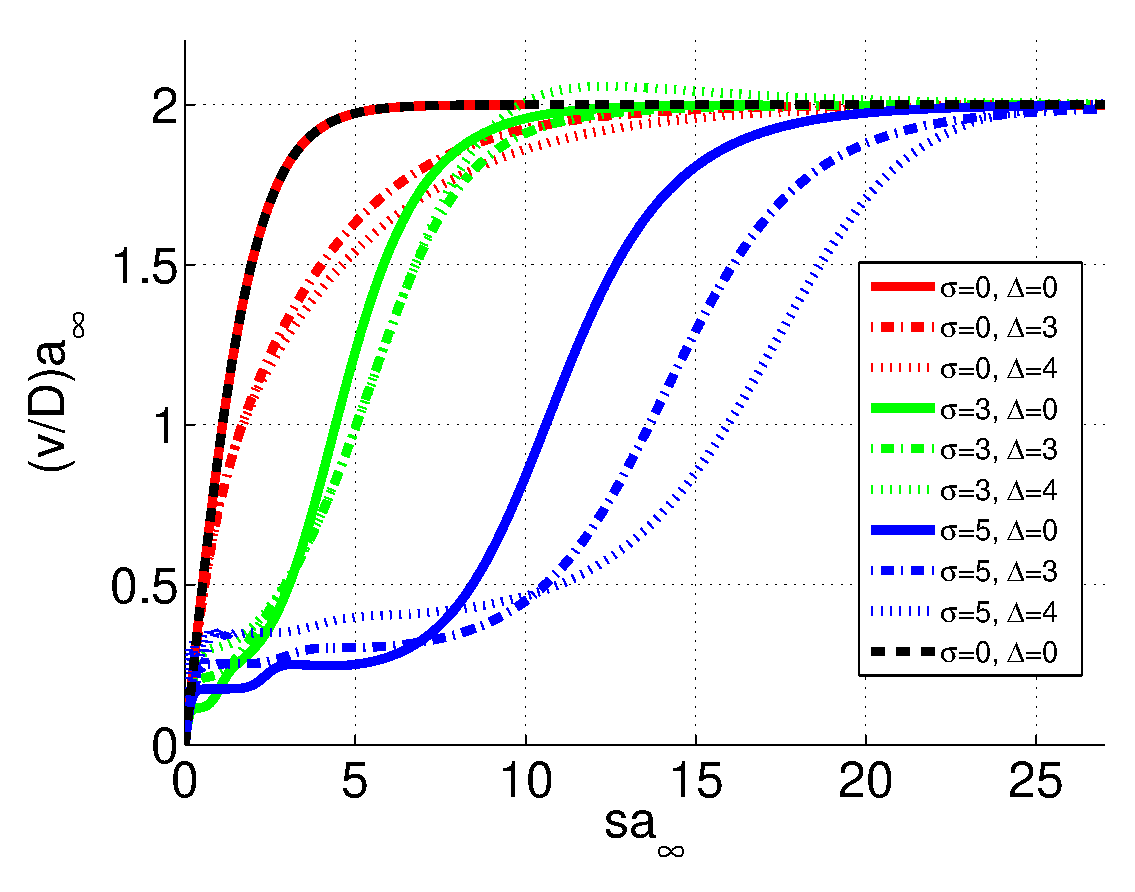
\includegraphics[height=7cm]{/Figs/vD.eps}

\caption{The Einstein relation scaled by the effective lattice constant $a_{\infty}v/D$
vs. the scaled affinity $x=a_{\infty}s$ for various values of $\sigma$ and $\Delta$.
Different colors correspond to different $\sigma$, different line styles correspond 
to different $\Delta$. 
The dashed black line is $2\tanh(x)$ corresponding to no disorder. 
}
\label{fig2}
\end{figure}


%\begin{figure}
%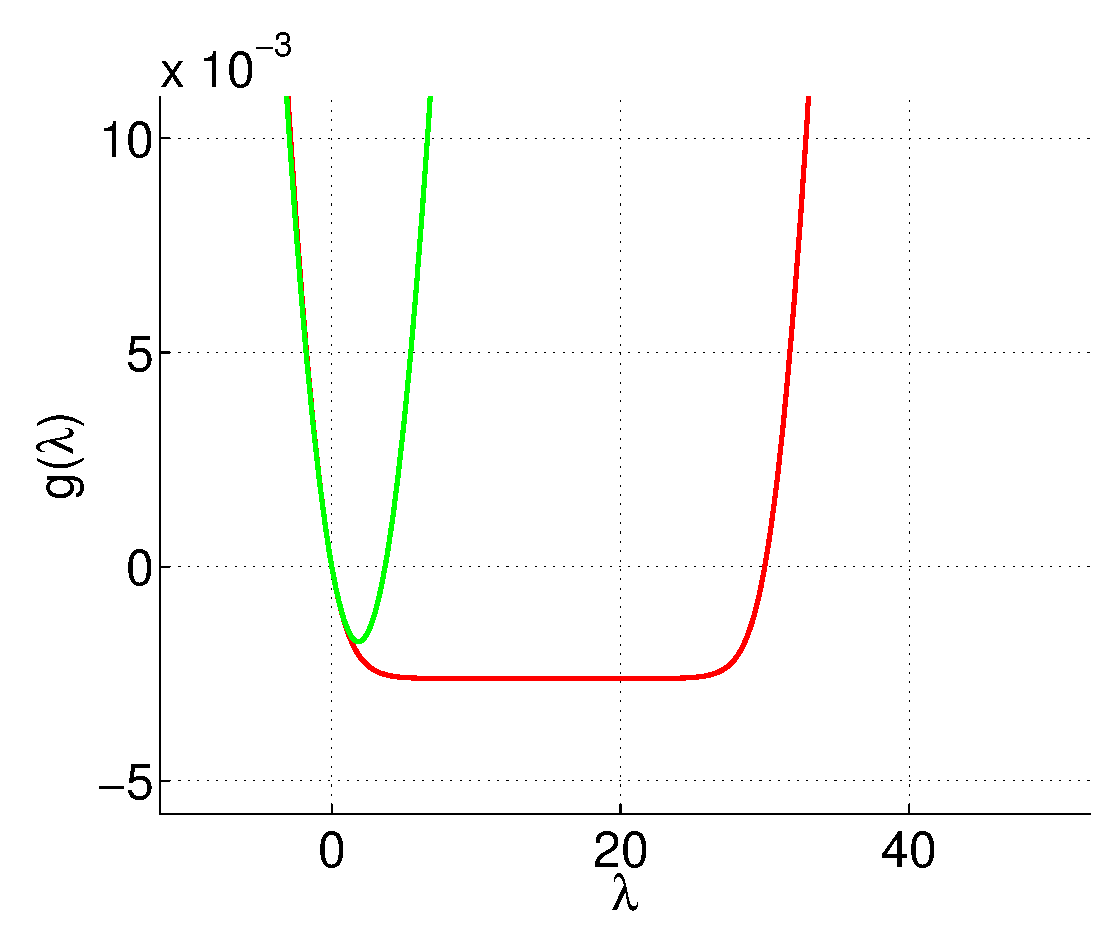
\includegraphics[height=6.5cm]{/Figs/g_Delta_3_Sigma_3_s_1.eps}
%\caption{The generating function for the winding number for $N=30$ sites (red line), 
%compared with the parabola defined by the same first and second moments.
%The parameter $h$ is the difference between minima.}
%\label{fig1}
%\end{figure}

\begin{figure}

%
%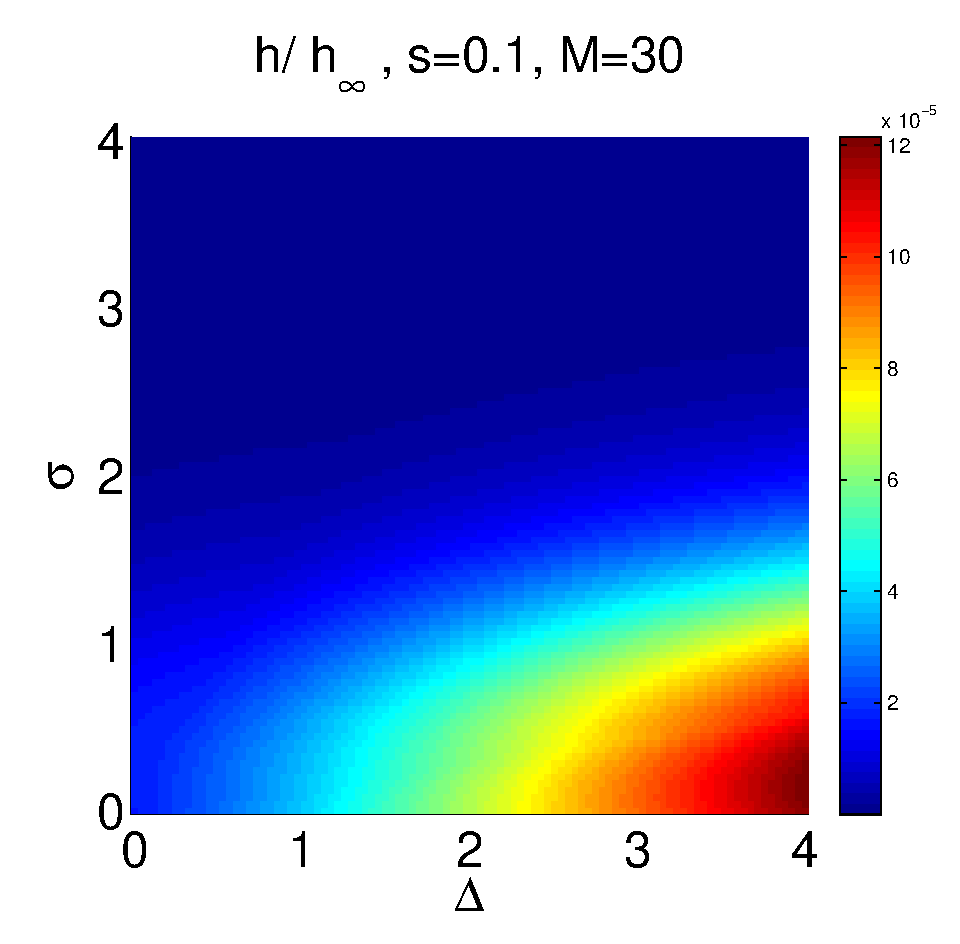
\includegraphics[height=4cm]{/Figs/h_hinf_1.eps}
%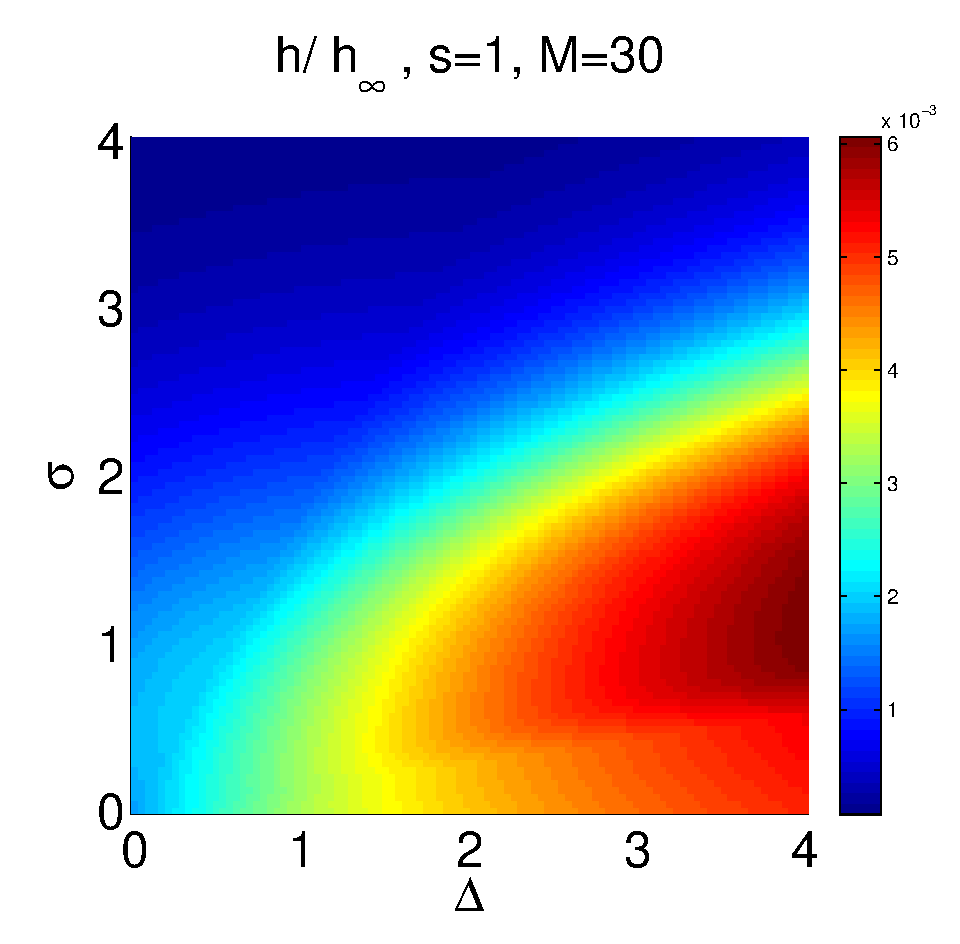
\includegraphics[height=4cm]{/Figs/h_hinf_2.eps}
%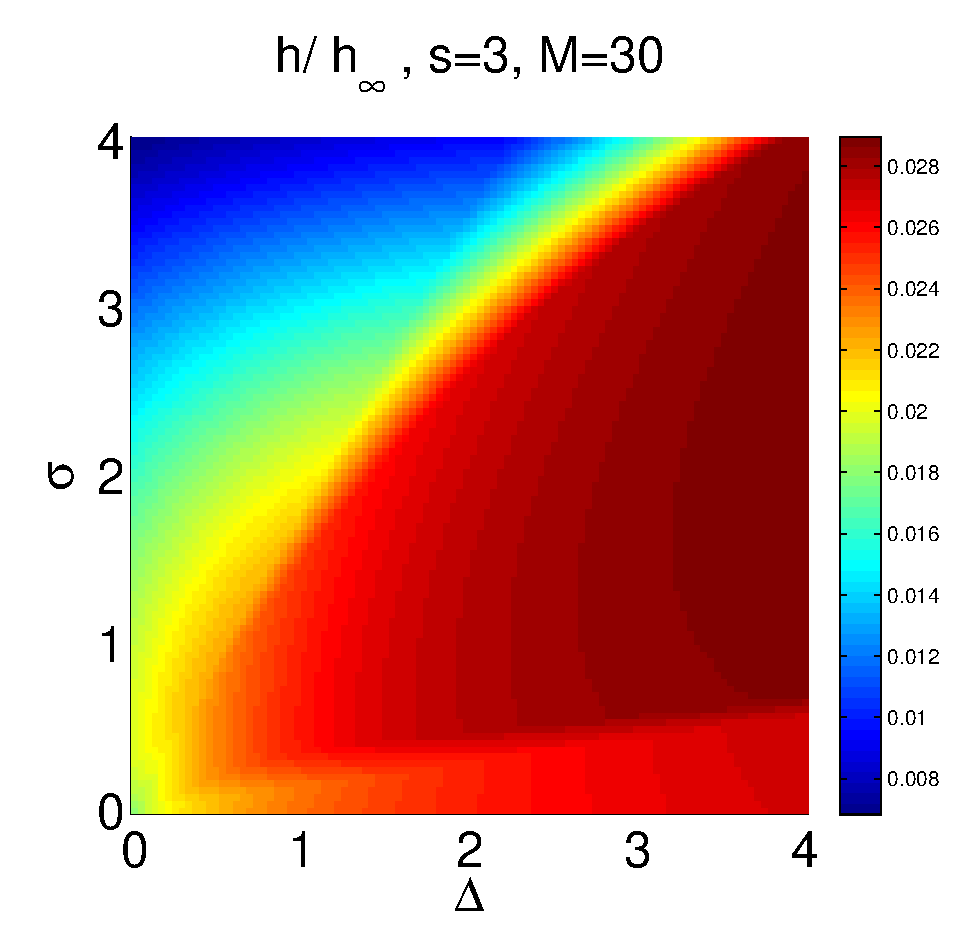
\includegraphics[height=4cm]{/Figs/h_hinf_3.eps}
%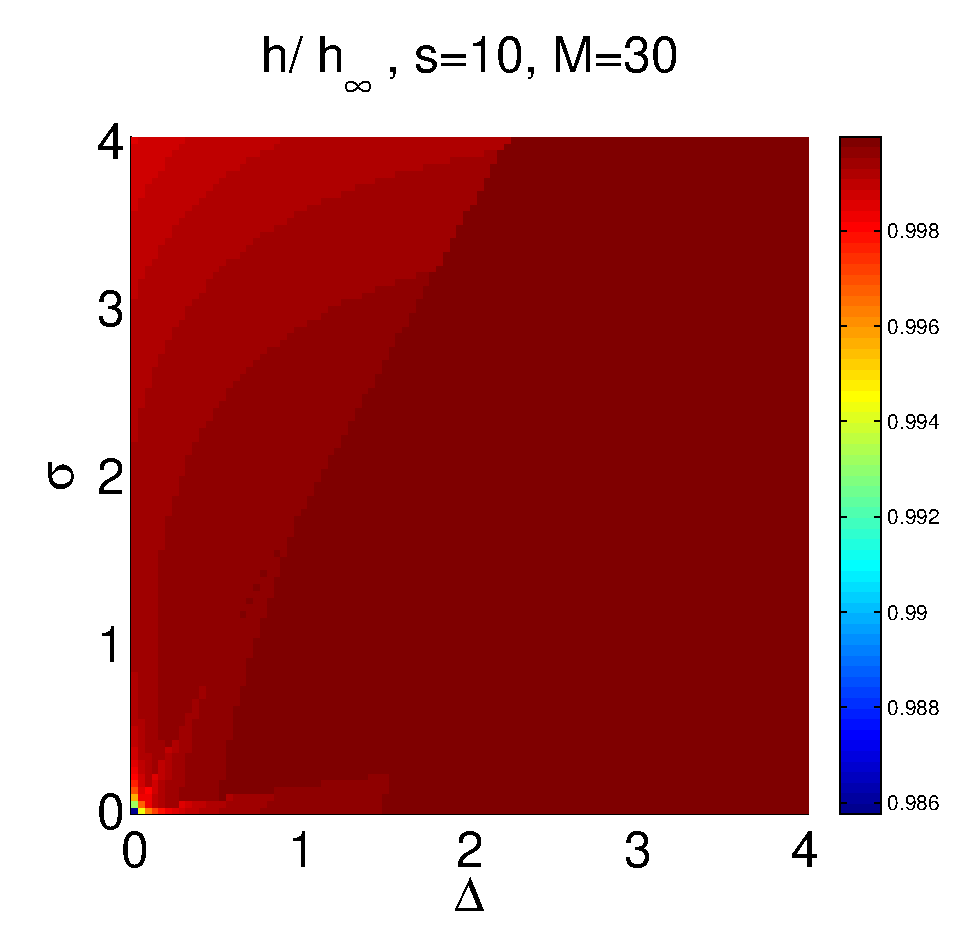
\includegraphics[height=4cm]{/Figs/h_hinf_4.eps}
%
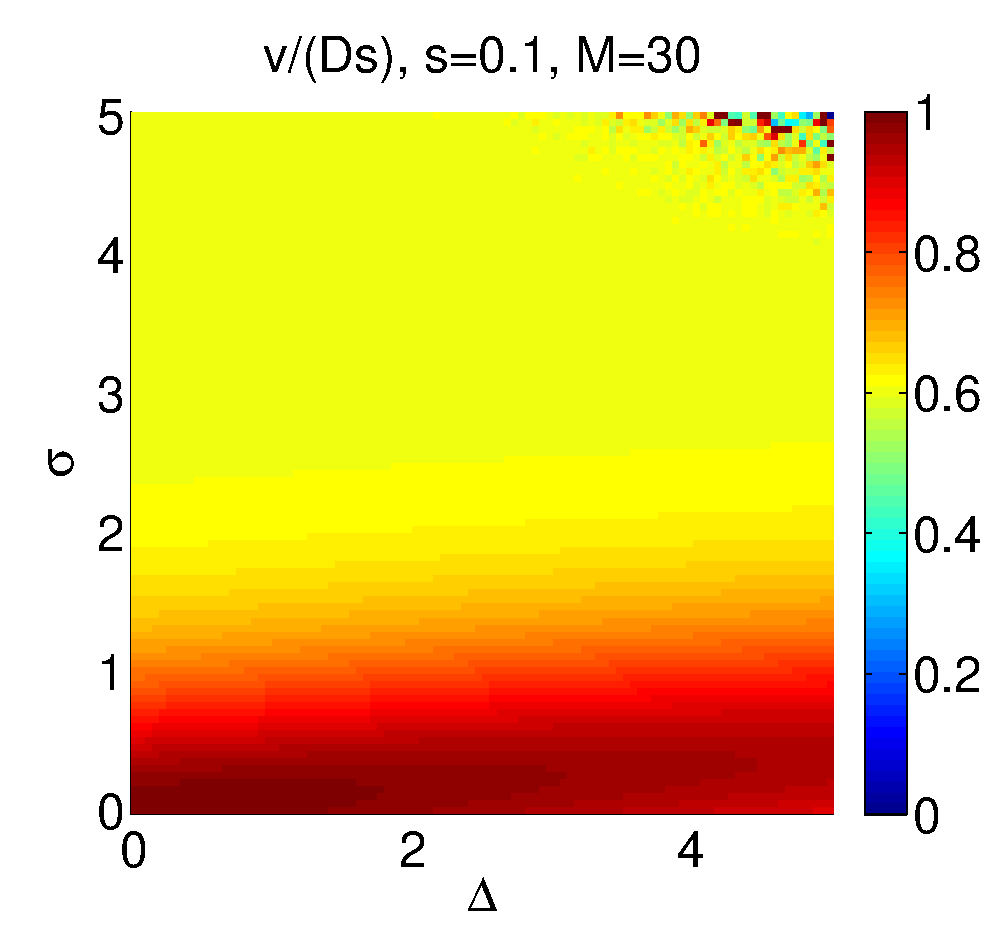
\includegraphics[height=4cm]{/Figs/vDs_1.eps}
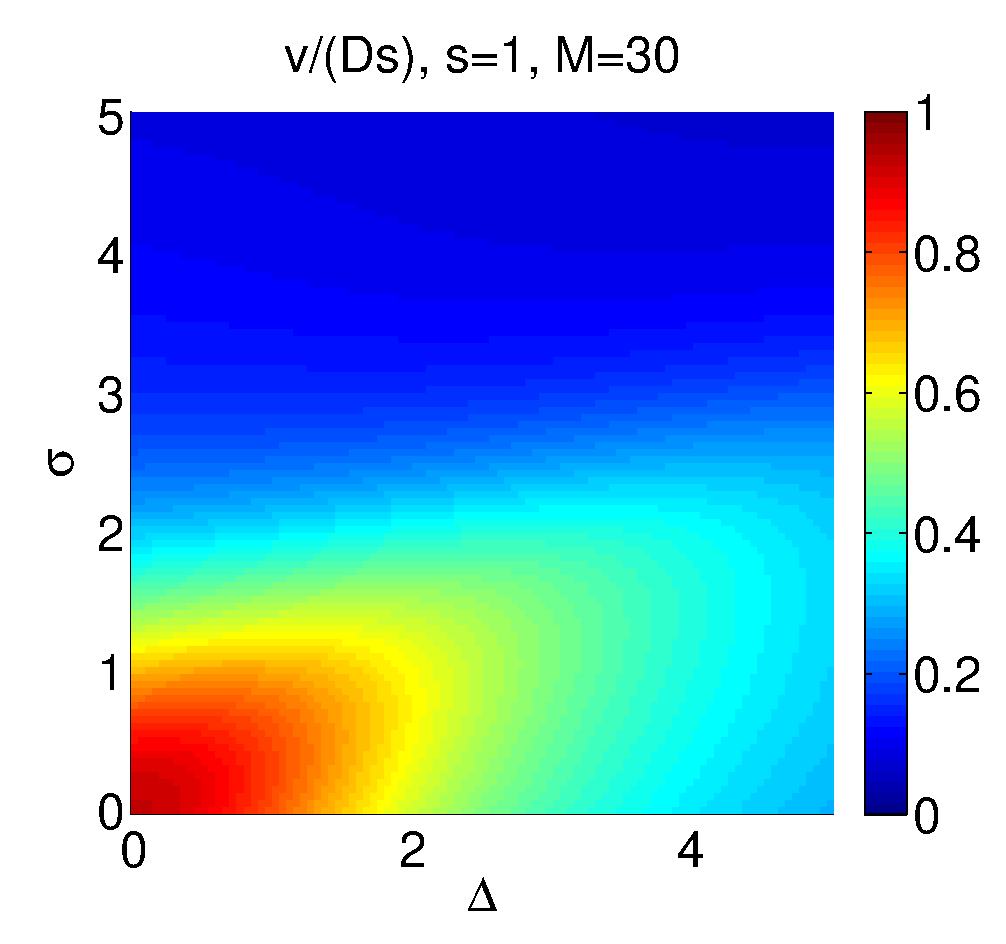
\includegraphics[height=4cm]{/Figs/vDs_2.eps}
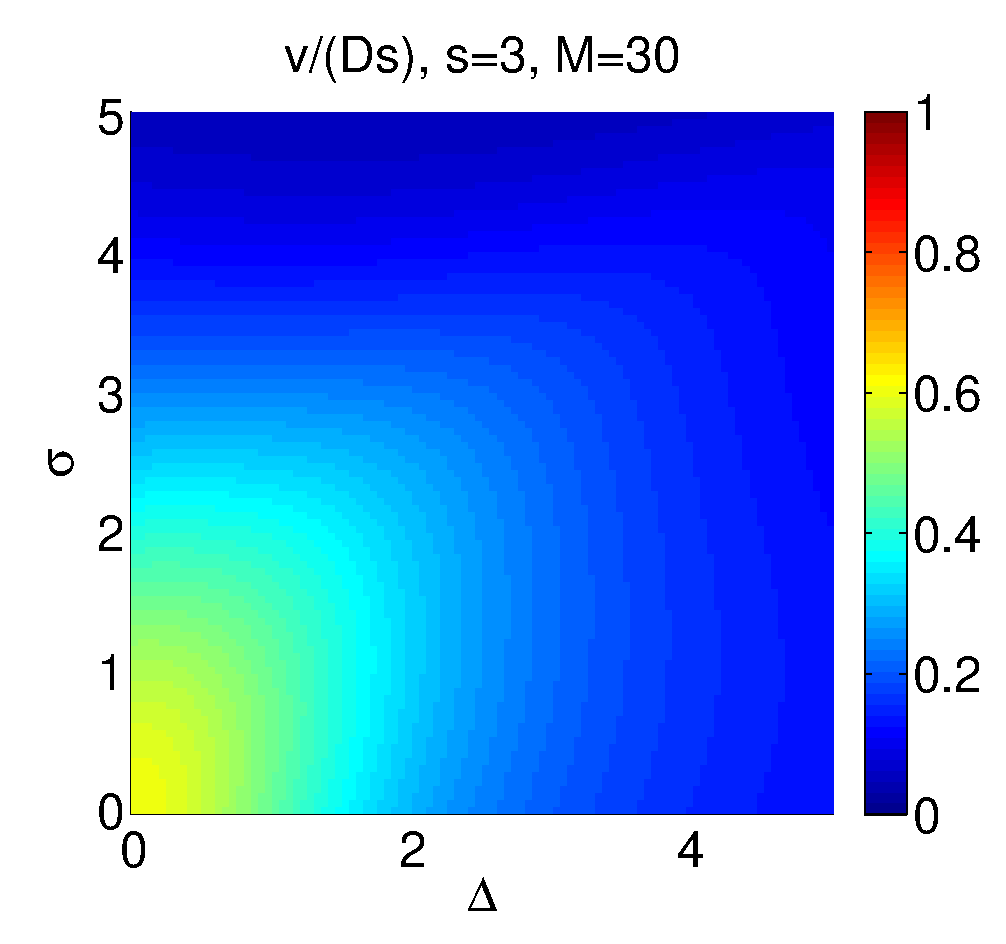
\includegraphics[height=4cm]{/Figs/vDs_3.eps}
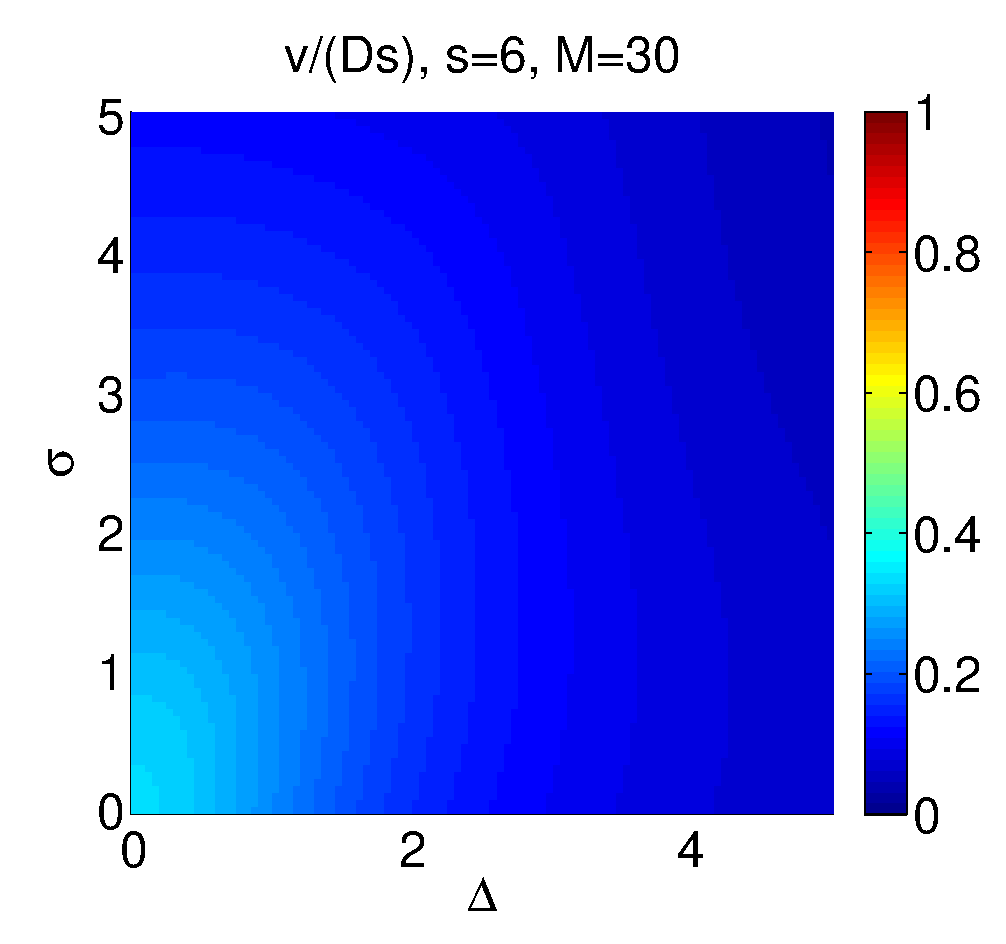
\includegraphics[height=4cm]{/Figs/vDs_4.eps}
%
%
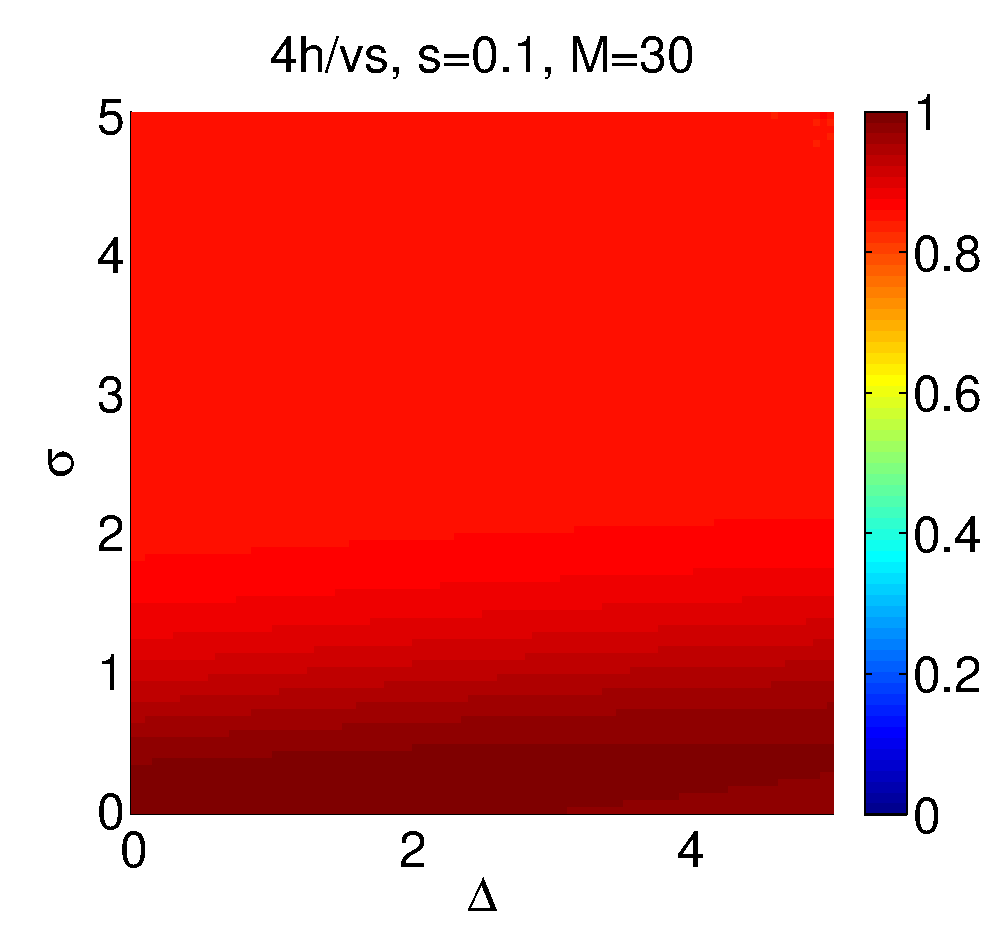
\includegraphics[height=4cm]{/Figs/vhs_1.eps}
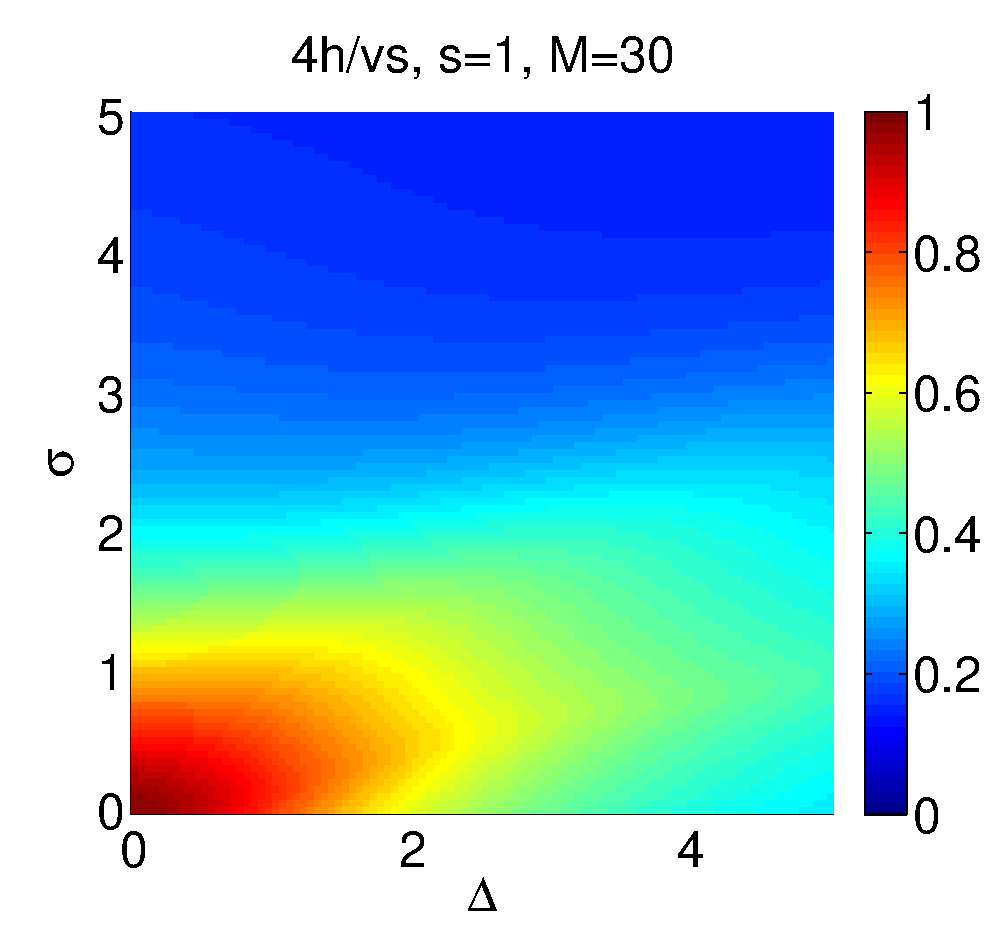
\includegraphics[height=4cm]{/Figs/vhs_2.eps}
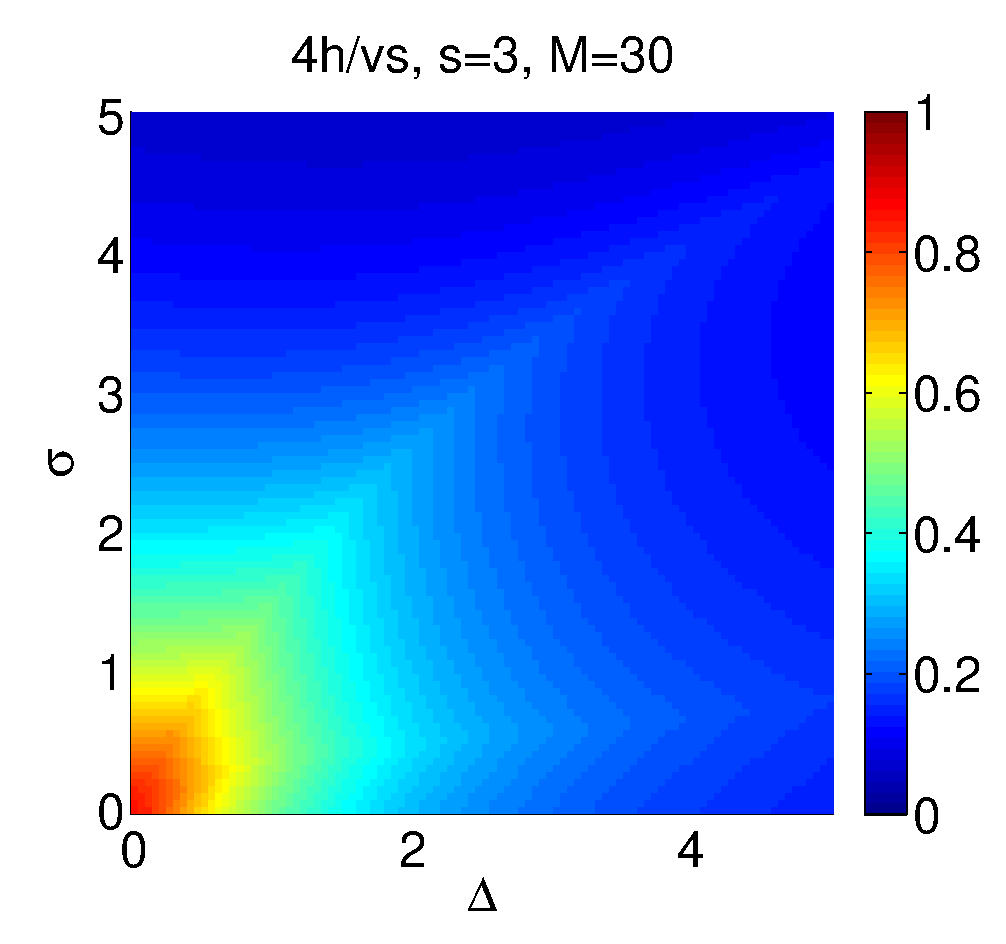
\includegraphics[height=4cm]{/Figs/vhs_3.eps}
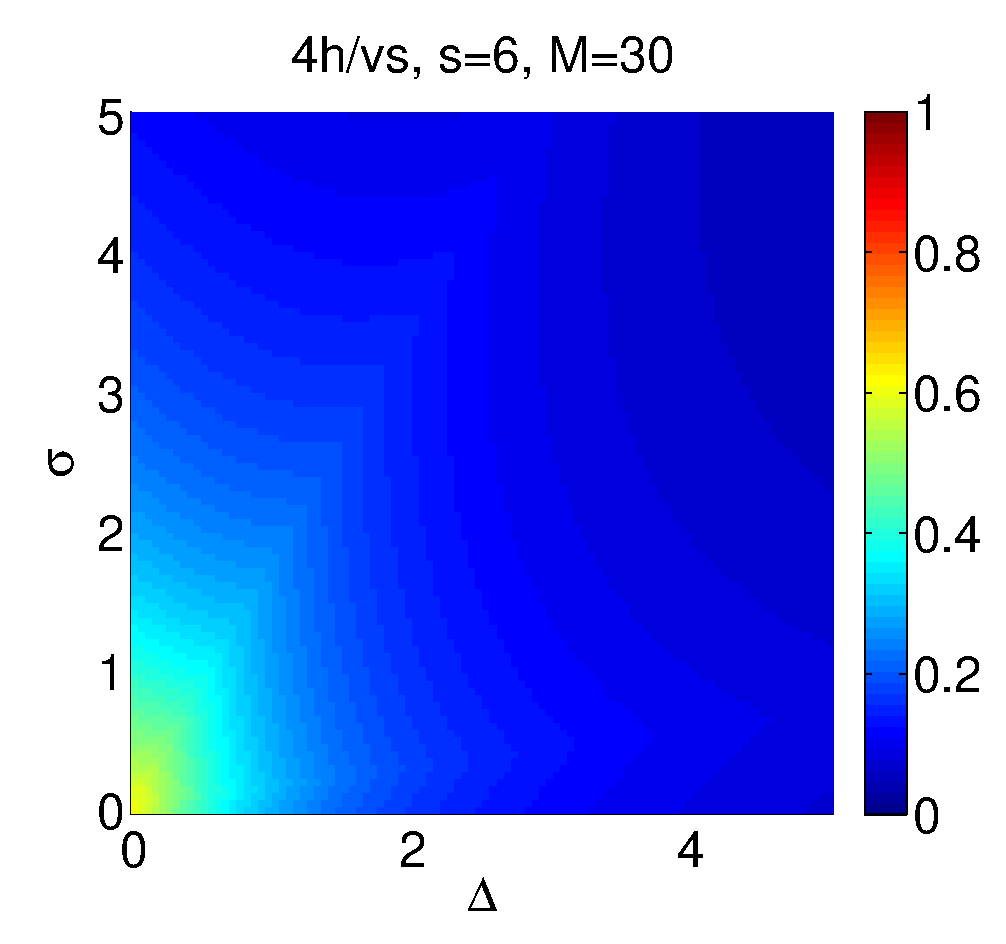
\includegraphics[height=4cm]{/Figs/vhs_4.eps}
%
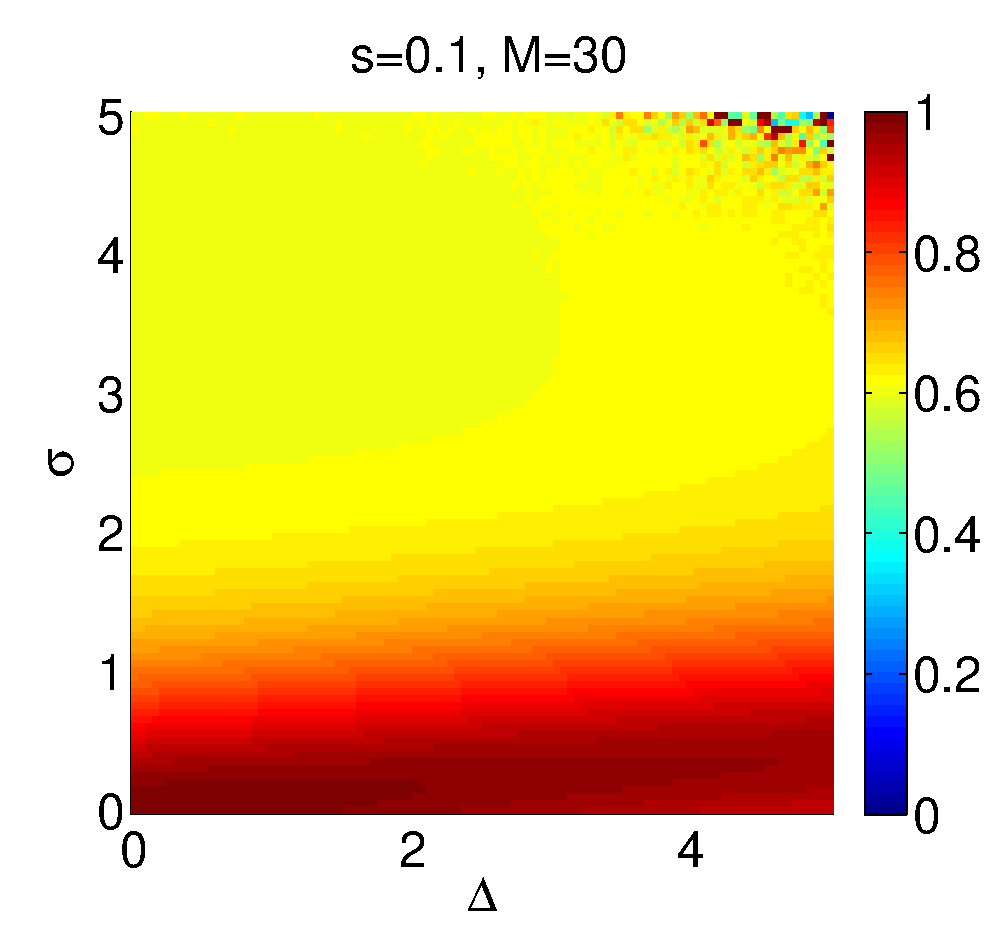
\includegraphics[height=4cm]{/Figs/vD_vDinf_1.eps}
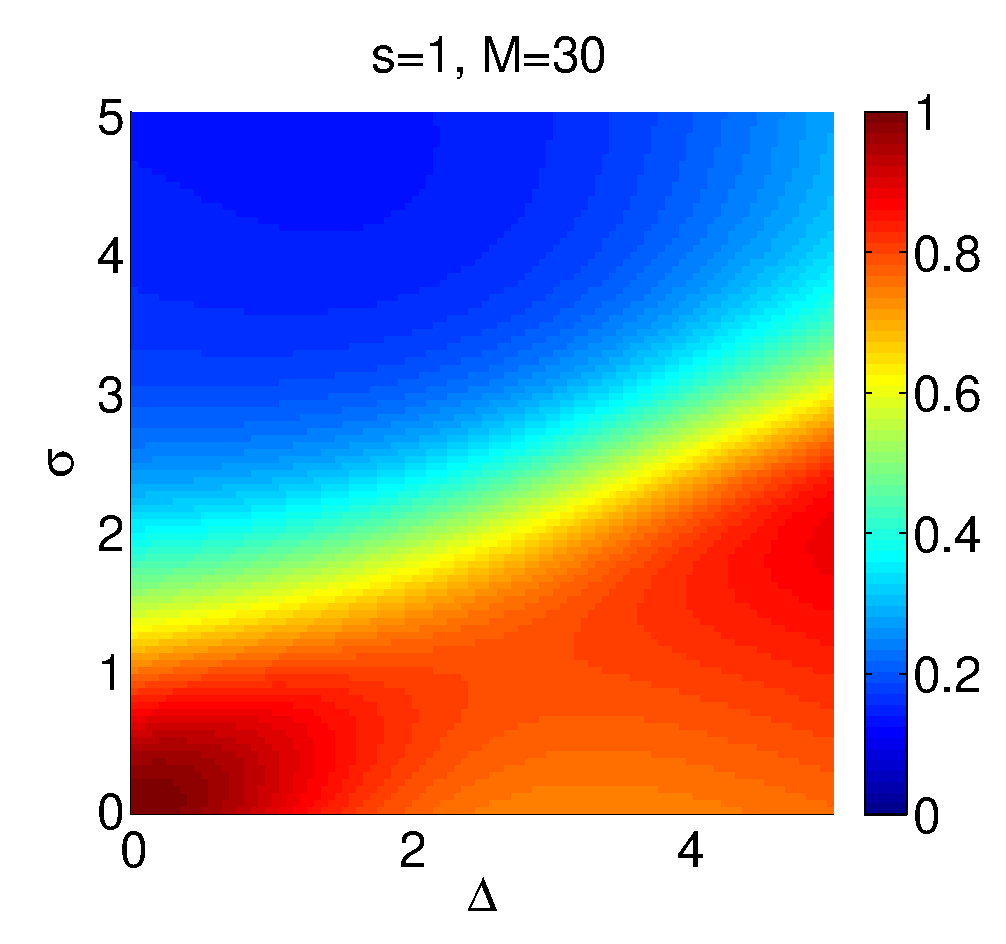
\includegraphics[height=4cm]{/Figs/vD_vDinf_2.eps}
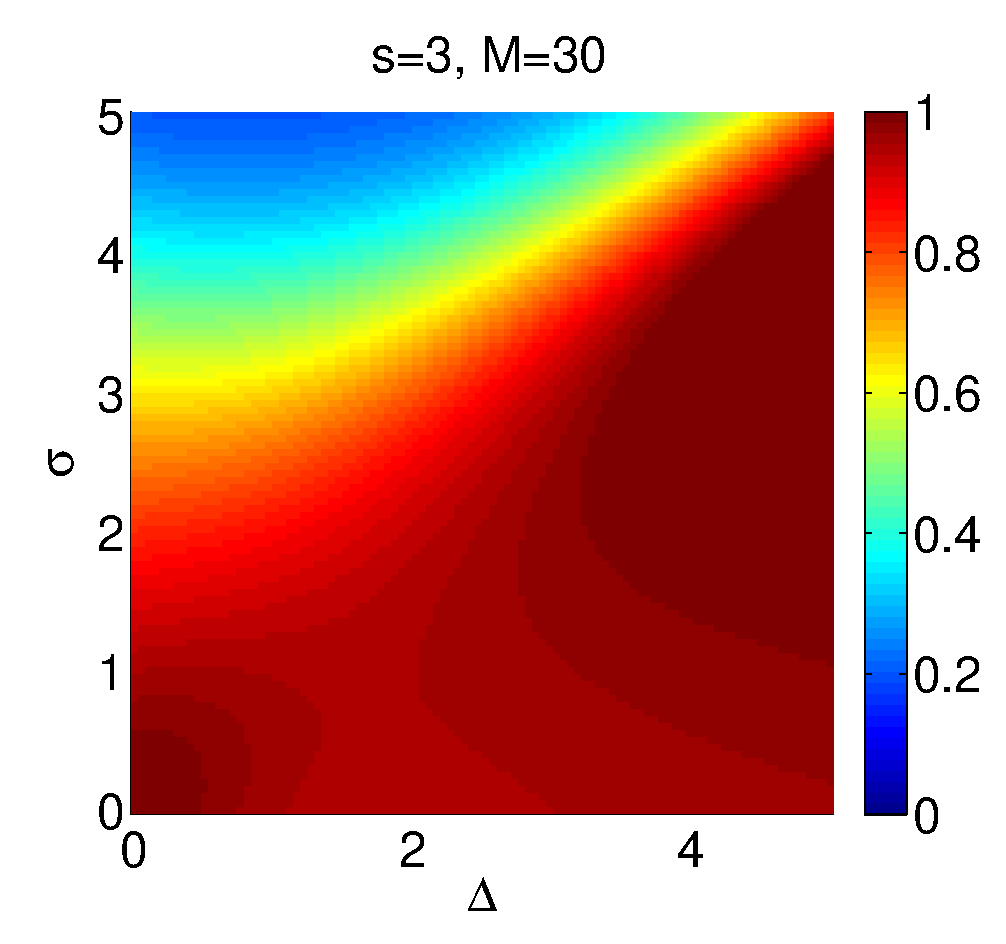
\includegraphics[height=4cm]{/Figs/vD_vDinf_3.eps}
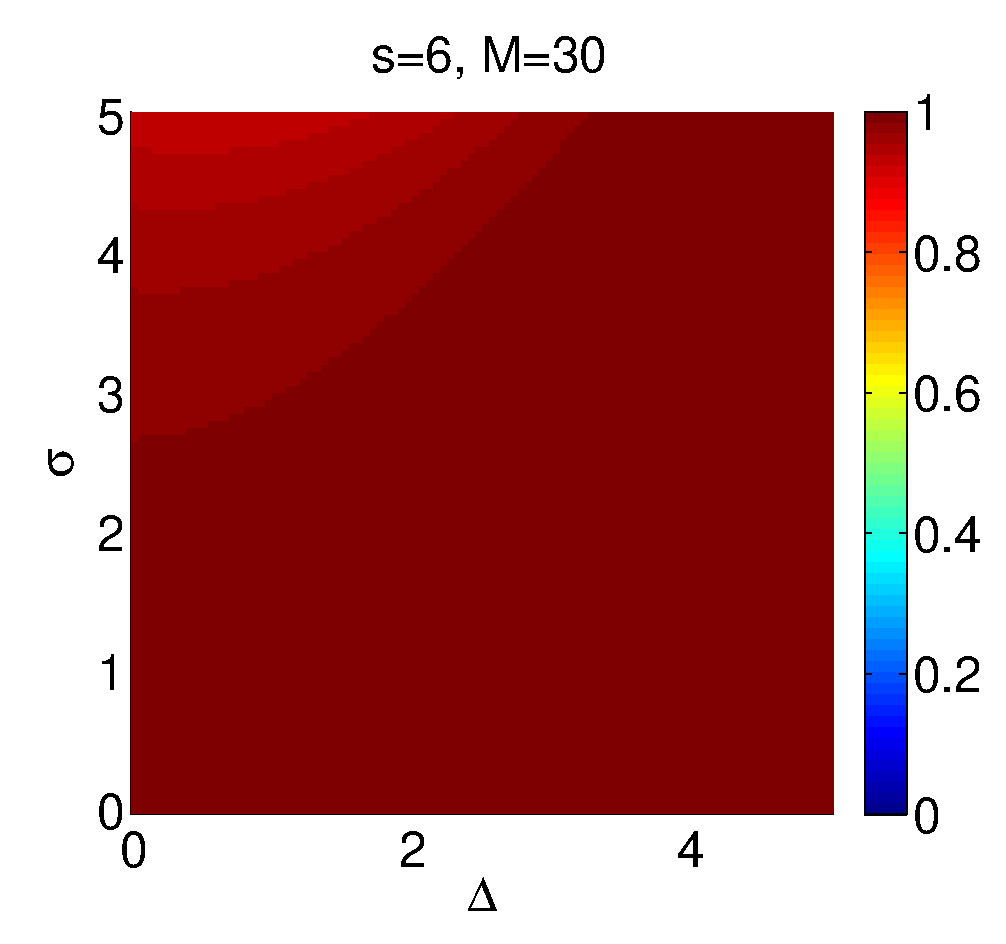
\includegraphics[height=4cm]{/Figs/vD_vDinf_4.eps}
%
%%
%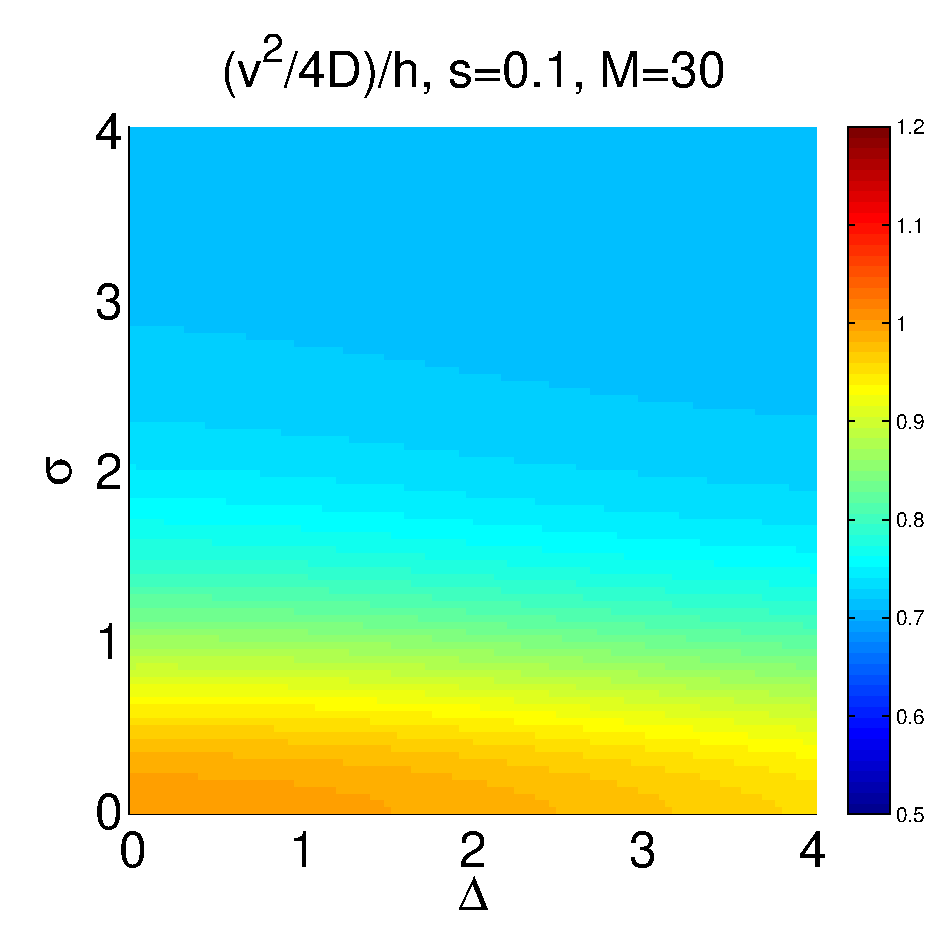
\includegraphics[height=5cm]{/Figs/hvD_s_1.eps}
%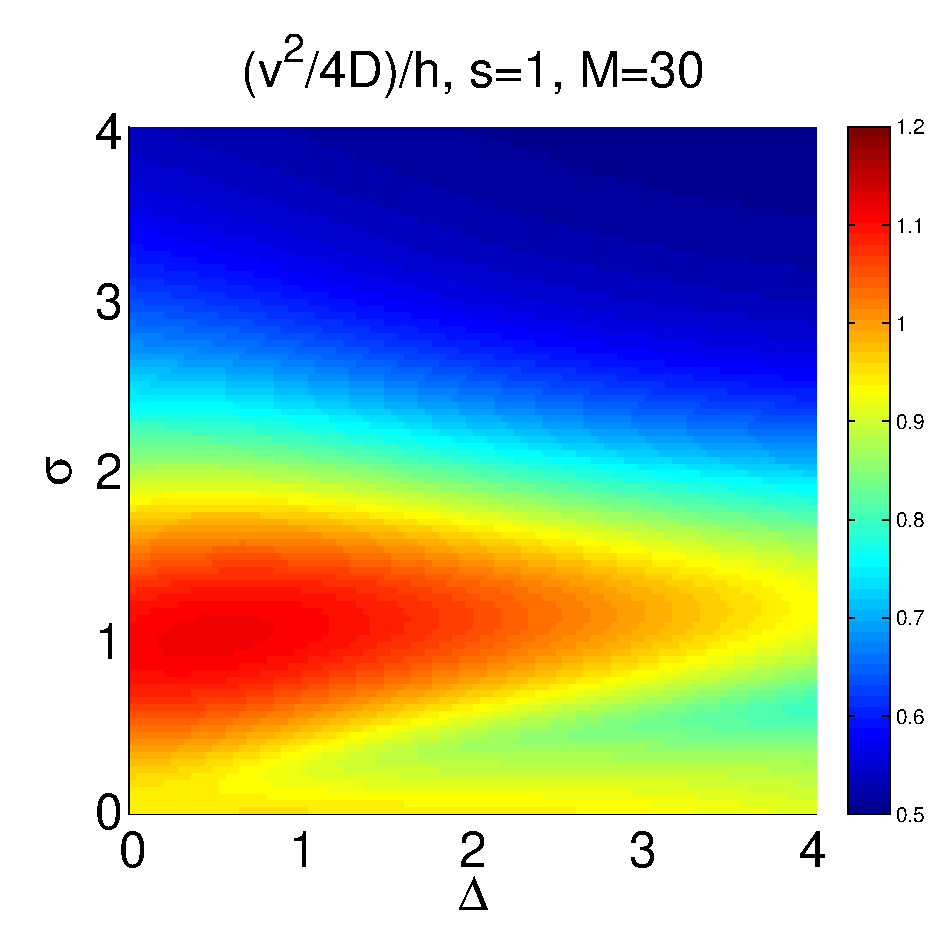
\includegraphics[height=5cm]{/Figs/hvD_s_2.eps}
%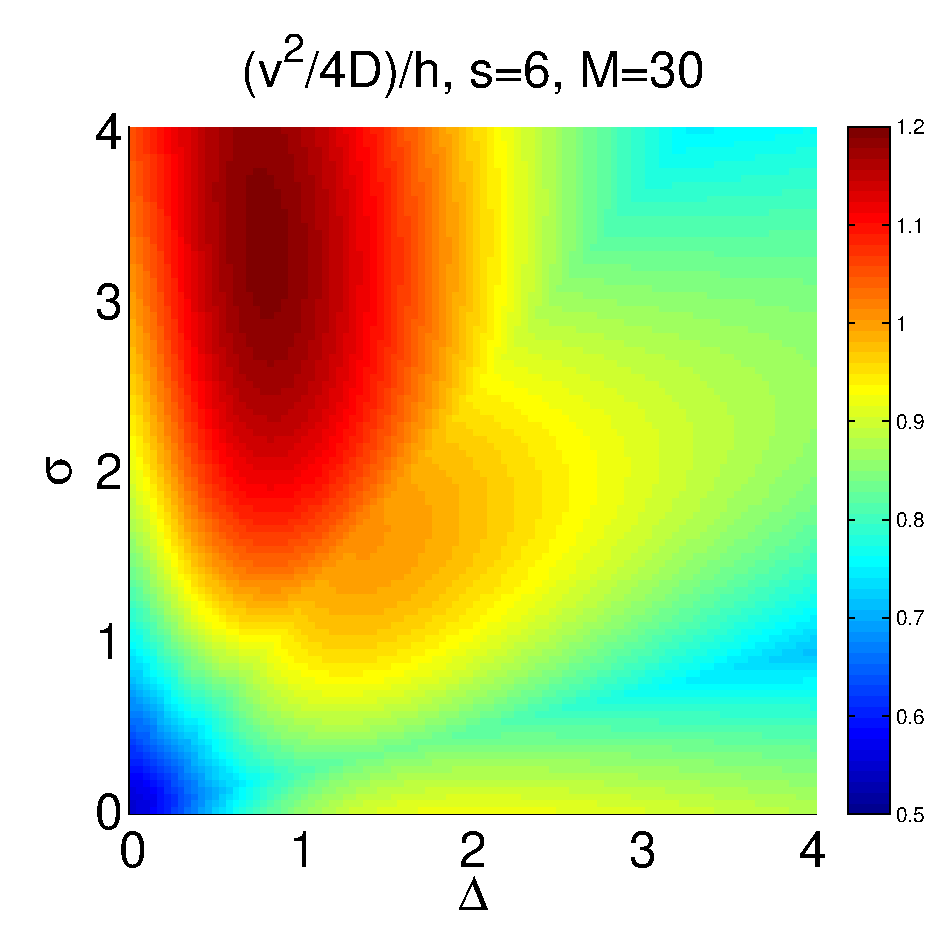
\includegraphics[height=5cm]{/Figs/hvD_s_3.eps}

\caption{
First row: The ratio of first to second moments, normalised by $s$.
Second row: Ratio of velocity to peak value $h$, normalised by $s$.
Third row: The ratio $ v/D $ divided by $2a_{\infty}^{-1}\tanh(a_{\infty}s/2)$.}
\label{fig3}
\end{figure}



\begin{figure}
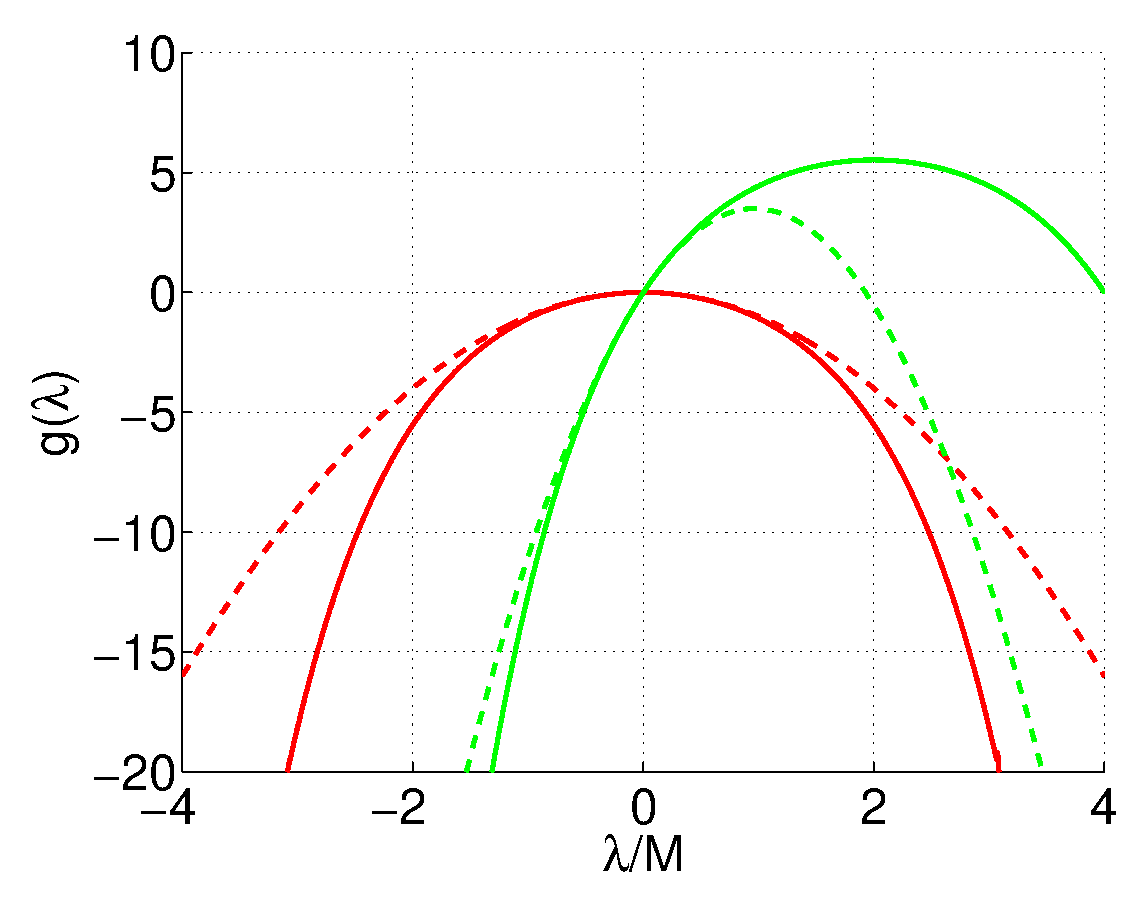
\includegraphics[height=7cm]{/Figs/g_lambda_M.eps}

\caption{The effect of discretization  on the generating function $g(\lambda)$.The red line is for $s=0$, the green line is for $s=4$. 
In both cases $\sigma=0$ and $\Delta=0$.
Dashed lines are parabolas $v\lambda - D\lambda^2$.
}
\label{fig4}
\end{figure}

\end{document}
%%%%%%%%%%%%%%%%%%%%%%%%%%%%%%%%%%%%%%%%%%%%%%%%%%%%%%%%%%%%%%%%%%
